

\documentclass[a4paper,11pt]{article} 
\usepackage[spanish]{babel}           
\usepackage[utf8]{inputenc}           

\usepackage[T1]{fontenc}   		   % Fonte por defecto.
\usepackage{graphicx, subfigure}    		   % Engadir imaxes.
\usepackage{color}      		   % Uso de cores.
\usepackage{anysize}     		   % Modificar o tamaño dos marxes.
\usepackage{multicol, multirow}    % Escribir a doble, triple...columna.
\usepackage{bm}          		   % Letras gregas en negriña.
\usepackage{textcomp}    		   % Símbolos, poden consultarse na rede.
\usepackage{eurosym}     		   % Símbolo € (\euro).
\usepackage{amsthm}                % Paquete da AMS para escribir teoremas.
\usepackage{amsmath,amsfonts}      %Paquetes específicos de símbolos.
\usepackage{lineno}                % Numerar as liñas. 

\marginsize{1.5cm}{1.5cm}{1.5cm}{1.5cm} % MARXES: Esq, der, sup, inf.
\parindent=0mm                        % Sangría. 
\parskip=2mm                          % Espazo entre párrafos.
\renewcommand{\baselinestretch}{1}    % Interliñado.
\renewcommand{\spanishtablename}{Táboa} 


\title{Tema 5: Memoria semántica e representación do coñecemento}
\date{} %Para que non apareza deixa o espaxo entre {} valeiro. Para que apareza a data de hoxe: \today


\begin{document}  

\maketitle 

\section{Memoria semántica e memoria episódica}
\begin{itemize}
	\item \textbf{Memoria semántica:} Memoria declarativa de coñecementos e feitos xerais, que non 
	fan referencia ó contexto no que se adquiriron (coñecemento sobre o mundo, vocabulario, regras 
	para resolver problemas...). Implica a ``consciencia de coñecer'' ou conciencia noética.
	\item \textbf{Memoria episódica:} Memoria para eventos que ocorren nun tempo e lugar 
	específicos. Durante o recordo revívense algúns aspectos do evento orixinal, através da 
	capacidade de recolección consciente, ou do chamado <<viaxe mental no tempo>>. Esta memoria 
	implica autocoñecemento ou conciencia autonoética.
\end{itemize}

Coñécense diferentes datos neuropsicolóxicos que demostran que estas dúas memorias son diferentes:
\begin{itemize}
	\item \underline{Amnesia}: Spiers, Maguire e Burgess (2001) revisan 147 casos de amnesia, 
	atopando danos de memoria episódica en todos eles. Porén, observan que moitos pacientes só 
	presentan pequenos problemas de memoria semántica. O impacto do dano cerebral é moito maior 
	sobre a memoria episódica que sobre a semántica.
	\item \underline{Amnesia retrógrada}: Fallo na retención da información adquirida antes da 
	aparición da amnesia. Tulving (2002) estuda o caso de KC, cuxa amnesia fora drasticamente peor 
	para a súa memoria episódica que para a semántica: o seu coñecemento semántico permanecía 
	razoablemente intacto, mentres que non podía recordar ningún evento persoal.
	\item \underline{Demencia semántica}: Os pacientes presentan problemas severos en memoria 
	semántica, pero manteñen relativamente intacta a memoria episódica. Este problema asóciase ó 
	dano na parte anterior dos lóbulos frontotemporais.
\end{itemize}

\section{Organización conceptual}
\subsection{Que tipo de información se almacena na memoria semántica?}
A memoria semántica recolle conceptos de varios tipos, cuxa forma de almacenamento hai que considerar.

Loftus (1972) realiza un experimento cunha tarefa na que os participantes deben atopar unha palabra específica, dadas a súa categoría e letra inicial. Observa que as respostas son máis rápidas cando se presenta primeiro a categoría (\textit{fruta}) e logo a letra (\textit{p}) que cando se fai o contrario. Isto suxire que é máis fácil activar a categoría e prepararse para buscar a palabra que buscar entre tódalas palabras que comecen por unha determinada letra. Isto pode ocorrer porque as categorías adoitan ser coherentes e manexables, mentres que o conxunto de palabras que comezan por unha letra específica adoita ser demasiado amplo e difuso. 

\subsection{Modelo de redes xerárquicas (Collins e Quillian, 1969)}
Propón que a memoria semántica se organiza nunha serie de redes xerárquicas, na que os conceptos principais se representan como nodos e hai propiedades ou características asociadas a cada concepto. A información de ditas propiedades almacénase o máis alto posible na xerarquía, para minimizar a cantidade de información retida: a organización neste sistema baséase no principio de economía cognitiva. 

Os investigadores poñen a proba o seu modelo mediante unha tarefa de verificación de frases, na que os participantes deben decidir se estas son verdadeiras ou falsas. No caso das verdadeiras, aumenta o tempo de verificación a medida que o fai a separación (xerárquica) entre o suxeito da frase e a propiedade que o acompaña. O modelo afirma, correctamente, que con frecuencia se emprega a memoria semántica para inferir as respostas correctas. 

Con todo, este modelo presenta varios problemas. En primeiro lugar, Conrad (1972) atopa que a verificación de moitas frases é máis lenta non pola distancia xerárquica entre os seus compoñentes, senon porque son pouco familiares. Cando se controla este factor, a separación xerárquica resulta ter moi pouco efecto sobre o tempo de verificación.

En segundo lugar, o modelo supón que tódolos membros das categorías son igual de sinxelos de identificar (\textit{exemplo:} un canario e un pingüín son paxaros). Porén, os membros da maioría de categorías non son igual de representativos, e o tempo de verificación é máis rápido no caso dos membros máis típicos e representativos que no dos máis atípicos. Isto é o que se denomina <<gradiente de tipicidade>>; Collins e Quillian non o teñen en conta no seu experimento.

Por último, sábese que os membros máis típicos dunha categoría, comparados cos menos típicos, posúen a maioría de características asociadas a dita categoría. Por tanto, os Collins e Quillian equivócanse ó afirmar que os conceptos que empregamos pertencen a categorías definidas rixidamente: as categorías determínanse de forma flexible.

\subsection{Modelo de propagación da activación (Collins e Loftus, 1975)}
Nace co obxectivo de solucionar os problemas surxidos do modelo anterior. Fronte á noción de xerarquías lóxicas, demasiado inflexible, Collins e Loftus propoñen que a memoria semántica se organiza en torno a relacións ou distancia semántica. Esta distancia pode medirse pedindo a un grupo de persoas que decida a relación entre determinados pares de palabras ou pedíndolles que xeren unha lista de palabras que inclúe tódolos membros posibles dunha categoría dada (os que máis se repitan serán os máis relacionados coa categoría).

Segundo a teoría, cada vez que unha persoa percibe ou pensa sobre un concepto actívase un nodo na memoria semántica. A activación propágase con máis forza cara os conceptos estreitamente relacionados con este, e máis debilmente cara os menos relacionados. Por conseguinte, o modelo predí o efecto de tipicidade.

Ademais, o modelo tamén predí un efecto de facilitación ou \textit{priming} semántico, que se produce cando unha palabra facilita o procesamento doutra (obxectivo) coa que está relacionada.

\subsection{Avaliación dos modelos}
A noción de que a activación se propaga entre os conceptos semanticamente relacionados resultou ser enormemente influinte. Ademais, o segundo modelo é máis flexible que o primeiro, o que supón unha vantaxe no sentido de que pode explicar máis feitos empíricos. 

Con todo, a flexibilidade do modelo de propagación tamén presenta desvantaxes ó reducir a especificidade das súas predicións, facendo que sexan máis difíciles de probar. 

Por último, o modelo de propagación propón que cada concepto almacenado na memoria semántica está representado por un só nodo. Esta idea é demasiado sinxela: en realidade, os diferentes tipos de información (visual, auditiva...) sobre cada obxecto almacénanse en diferentes rexións cerebrais. 

\section{Esquemas mentais}
\subsection{Características}
\begin{itemize}
	\item \textbf{Unidades cognitivas de alto nivel:} Os esquemas son entidades conceptuais 
	complexas compostas de unidades máis sinxelas. Adoitan incluir unha serie de peroaxes, obxectos, 
	accións, metas, etc.
	\item \textbf{Encáixanse uns noutros:} O sistema de coñecemento humano consiste nun conxunto de 
	esquemas interconectados. Cada esquema integra outros máis elementais e constitúe un subesquema 
	doutro. Esta disposición xerárquica está limitada, xa que seguramente existen esquemas atómicos 
	ou primitivos que non poden descompoñerse en subesquemas.
	\item \textbf{Actualizables:} Os esquemas son paquetes de coñecementos prototípicos cuxas 
	variables non están especificadas. Os valores destas variables modifícanse en función do 
	contexto. A actualización dos esquemas xera interferencias temáticas, a través do mecanismo de 
	encher valores ausentes.
	\item \textbf{Multifuncionais:} A utilidade teórica dos esquemas é moi ampla. Guían os procesos 
	de comprensión e percepción visual, analizando a información a partir do seu contido e tentando 
	que esta información encaixe neles. Tamén revolucionaron o estudo da memoria, que se considera 
	un subproduto da activación dos esquemas durante a comprensión de textos e durante a 
	recuperación. Ademais controlan o comportamento, en especial os patróns condutuais complexos.
\end{itemize}

Non se coñece o mecanismo exacto de indución de esquemas, pero parece que a capacidade de xeralos é unha habilidade básica que se desenvolve moi pronto nos individuos.

\subsection{Tipos de esquemas}
Existe unha gran diversidade de coñecementos que se poden representar mediante esquemas. Practicamente tódolos contidos da memoria se organizan total ou parcialmente en esquemas.

\begin{itemize}
	\item \underline{Esquemas visuais (marcos)}: Interveñen na comprensión de símbolos e nos 
	procesos perceptivos habituais. A percepción visual é unha operación con varios niveis, un máis 
	sinxelo, que implica procesos automáticos paralelos, e un de agrupamento de características que 
	permite configurar obxectos e esceas, e que implica esquemas interpretativos que se coñecen como 
	<<marcos>> (Minsky, 1975). Cada marco contén información prototípica, polo que cada escea inclúe 
	un sistema de marcos que se van activando a medida que o observador se despraza polo medio. Os 
	marcos funcionan igual que os esquemas, e é posible simulalos en programas informáticos.
	\item \underline{Esquemas situacionais (guións)}: Paquetes de información relativos a situacións 
	convecionais. Inclúen persoaxes, obxectos e accións asociados a cada experiencia. Schanck e 
	Abelson (1977) desenvolven a idea de <<guión>> como analoxía do marco, aínda que o obxectivo do 
	primeiro é a comprensión de historias, en lugar da de esceas visuais.
	
	O guión recolle unha secuencia estereotipada de accións ordeadas, que manteñen entre si unha 
	dependencia causal. Inclúe as perspectivas das diferentes persoaxes e presenta diversos graos de 
	abstracción (desde máis xenérico a máis específico). Os guións son estereotipos culturais 
	compartidos cuxa estrutura interna, como a das categorías naturais, é difusa. Porén, non tódolos 
	eventos son igual de representativos dentro do guión: os considerados máis típicos ou centrais 
	son os máis compartidos pola poboación.
	
	Os guións interveñen na comprensión de textos, axudando a entender máis do que aparece explícito 
	neles, na codificación e no recordo. Ademais, teñen valor prescritivo ó aportar información 
	sobre os patróns de conduta aceptables en situacións convencionais.
	\item \underline{Esquemas de dominio}: Kintsch e Van Dijk (1978) introdúcenos no seu modelo de 
	comprensión de textos. Son esquemas moi abstractos que guían a comprensión e produción de 
	discursos, especialmente cando estes son moi longos, ó xerar expectativas sobre a súa estrutura 
	e contidos.
	\item \underline{Esquemas sociais}: Abarcan unha dimensión sociocultural, recollendo a gran 
	parte do noso coñecemento referida a contidos interpersoais. Estes esquemas posúen información
	tipos de situacións interpersoais, tipos de persoas e individuos concretos, polo que permiten 
	predicir comportamentos, planificar a conduta, inferir motivacións alleas... Considiramos varios 
	tipos:
	\begin{itemize}
		\item[-] \textit{Esquemas xenéricos} ou prototipos de persoas, que interveñen na 
		codificación e recordo de \textit{impresións} sobre persoaxes concretas.
		\item[-] \textit{Temas de roles}, que permiten comprender e ter expectativas sobre as metas 
		e accións dos individuos; \textit{temas interperoais}, relativos a relacións sociais e 
		afectivas, que permiten comprender e predicir os propósitos e a conduta dos demais; e 
		\textit{temas vitais}, que describen os obxectivos vitais das persoas e son moi xerais, 
		abarcan temas interpersoais e condicionan a elección de metas.
		\item[-] \textit{Teorías implícitas}, tipo de esquemas que median na nosa comprensión e 
		conduta social (segundo algúns psicólogos sociais).
		\item[-] \textit{Ideoloxías e sistemas de crenzas}, tipo de esquemas cun ámbito de 
		aplicación moi amplo.
	\end{itemize}	
	\item \underline{Esquemas de autoconcepto}: Tipo de esquemas sociais que recollen o coñecemento 
	dun individuo sobre si mesmo (destrezas, debilidades, preferencias, temperamento...). 
	Loxicamente, as diferenzas individuais nestes esquemas son moi notables. 
	
	Un tipo de esquemas de autoconcepto destacado son os \textit{esquemas de xénero ou sexo}. Na 
	maioría de culturas existe un perfil diferencial entre homes e mulleres relativo a 
	comportamentos, roles e actividades, que aparece en idades moi temperás. Percíbese ós demais 
	segundo os patróns dun esquema sexual e moitos individuos compórtanse, percíbense a si mesmos e 
	pensan como masculinos ou femininos, constituíndo catro tipos de individuos:
	\begin{itemize}
		\item \textbf{Esquemáticos masculinos:} Inclúen no seu autoconcepto características como 
		<<ambición>>, <<asertividade>>, <<competitividade>>, etc.
		\item \textbf{Esquema feminino:} Inclúen no seu autoconcepto características como 
		<<amabilidade>>, <<cariño>>, <<delicadeza>>, etc.
		\item \textbf{Altos andróxinos:} Inclúen no seu autoconcepto características do esquema 
		masculino e do feminino.
		\item \textbf{Baixos andróxinos:} Non posúen elementos do esquema masculino nin do 
		feminino, sendo non esquemáticos respecto ó sexo. 
	\end{itemize}
	
	O tipo de esquema sexual asumido no autoconcepto determina como o suxeito procesa información 
	ambiental. 
\end{itemize}

\subsection{Funcionalidade dos esquemas}
\subsubsection{Na memoria}
\begin{itemize}
	\item \textbf{Memoria de textos:} Existen dúas hipóteses alternativas que postulan mecanismos 
	diferentes nesta memoria:
	\begin{itemize}
		\item \underline{Hipótese abstractiva}: Na memoria almacénase un resumo do texto, que é o 
		que recorda o suxeito posteriormente. Ante unha narración, o suxeito constrúe un texto base 
		composto por proposicións relacionadas. Ó mesmo tempo, activa os seus esquemas para que
		guíen a aplicación de regras sobre o texto base. Estas seleccionan as proposicións 
		relevantes dacordo co esquema e eliminan as irrelevantes. Como resultado obtense un texto 
		máis reducido e abstracto, que se incorpora á memoria do suxeito.
		
		A hipótese predí sobre todo erros de omisión. Asume que a memoria humana é moi fiel e está 
		dirixida á reprodución de información.
		\item \underline{Hipótese reconstrutiva}: O suxeito introduce información dos seus esquemas 
		durante a aprendizaxe do texto, polo que o recordo é produto dunha reconstrución activa. 
		Esta hipótese concibe a memoria como un sistema orientado a elaborar interpretacións 
		coherentes do pasado. Cando recordamos, acomodamos a información pasada ó noso coñecemento 
		actual. Se non hai incongruencias entre estes dous tipos de información, o recordo será 
		fiel. En caso contrario, poden producirse distorsións importantes no recordo. 
		
		A reconstrución opera no recordo guiado por esquemas e na comprensión, realizando 
		inferencias para encher os valores ausentes do esquema. Cando o paso do tempo debilita a 
		información na memoria ou cando o texto orixinal é incongruente, aumenta a probabilidade de 
		que se produzan distorsións reconstrutivas.
		\item \underline{Experimento de Spiro (1977)}: Indica que o deseño das tarefas experimentais 
		minimiza a aparición de reconstrucións, por varios motivos: empréganse textos estruturados e
		coherentes; os textos son ficticios, polo que o suxeito non se implica no tema; o tempo 
		entre a lectura do texto e a súa recuperación é moi breve; a finalidade explícita da tarefa 
		é a reprodución correcta do texto.
		
		Así, Spiro deseña unha tarefa experimental para a que elabora dúas historias cunha parte 
		común. Bob e Margie son dous mozos namorados que se coñeceron estudando. Bob plantéalle a 
		Margie que el non quere ter fillos. A partir daquí, as historias difiren: na versión 
		<<equilibrada>>, Margie coincide con Bob; na <<desequilibrada>>, Margie quere ser nai. 
		
		Parte dos suxeitos sabe que se trata dun experimento de memoria, e o resto cre que a 
		historia é real e que se van avaliar as súas reaccións ante as relacións interpersoais. Tras 
		a lectura, Spiro dalles a algúns suxeitos información auxiliar, que pode ser consistente ou 
		inconsistente coa historia. Realiza as probas de memoria dous días, tres semanas ou seis 
		semanas despois da lectura. Obtén unha porcentaxe de erros de reconstrución moi superior nos 
		suxeitos implicados persoalmente coa historia que recibiran información auxiliar 
		inconsistente (o 45\% de individuos cometen erros). 
		
		Os resultados amosan que os grupos con instrucións de memoria teñen un recordo máis preciso 
		porque se distancian da información contida no texto. En cambio, os implicados persoalmente 
		coa historia adoitan acomodar os relatos ás súas crenzas, xerando distorsións 
		reconstrutivas.
	\end{itemize}
	\item \textbf{Memoria de sucesos congruentes e incongruentes co esquema:} 
	\begin{itemize}
		\item \underline{Énfase na función selectiva}: Un esquema activado traballa como un 
		dispositivo de selección atencional, procesando a información que encaixa con el 
		(congruente) e ignorando a irrelevante.
		\item \underline{Énfase na distintividade}: A distintividade dun suceso sobre un conxunto de 
		sucesos máis convencionais incrementa a demanda de recursos cognitivos e a profundidade de 
		procesamento de dito suceso. O procesamento profundo produce trazos de memoria máis 
		persistentes, polo que se recordará mellor a información discrepante ou incongruente.
		\item \underline{Hipótese esquema+corrección}: Sostén que o receptor dunha fonte complexa de 
		información constrúe dous tipos de representacións, unha xenérica (información convencional) 
		e outra máis detallada (información discrepante). A actuación de diferentes mecanismos 
		provoca que os sucesos congruentes se codifiquen de forma pouco elaborada, integrándose no 
		esquema activado. Así, o seu recordo será alto, e o seu recoñecemento baixo. Pola contra, a 
		información novidosa recibirá máis atención e un procesamento máis elaborado e específico. 
		Así, o seu recordo será baixo, e o seu recoñecemento alto. Os datos experimentais confirman 
		esta hipótese.
	\end{itemize}
\end{itemize}

\subsubsection{Na acción}
Ademais de conter información conceptual sobre o mundo, os esquemas posúen un carácter procedimental, dirixido á acción. Guían a execución de patróns de conduta cara metas ambientais e permiten interpretar a conduta allea.

Aínda que tódolos esquemas conteñen un compoñente procedimental, algúns especialízanse na conduta. Estes chámanse <<esquemas de accións>> ou <<plans>>, e comparten as seguintes propiedades:
\begin{itemize}
	\item[-] Requiren un axente, xeralmente asociado a un esquema ou rol social.
	\item[-] Diríxense a metas ambientais.
	\item[-] Actívanse ante as intencións, que son estados internos.
 	\item[-] Organízanse xerarquicamente; plans de alto nivel, dirixidos a metas xerais, controlan
 	a actividade doutros subordinados, dirixidos a metas instrumentais. 
	\item[-] Inclúen métodos, secuencias de acción motrices necesarias para acadar a meta.
	\item[-] Están fortemente guiados por datos, isto é, a súa execución require retroalimentación 
	constante. Cada acción do esquema precisa que se satisfagan, antes da súa execución, certas 
	condicións ambientais.
\end{itemize}

Os esquemas de acción diferéncianse no seu grao de automatismo. Algúns son rutinarios, inclúen secuencias fixas e sobreaprendidas de acción, destinadas a acadar o mesmo conxunto de metas instrumentais. A vantaxe deste automatismo é que unha vez se activa a intención de acadar a meta, o plan execútase sen case prestar atención. O control activo durante a execución do plan pasa a depender de parámetros ambientais.

Outros plans non están tan determinados, xa que podemos atoparnos con metas novas en situacións pouco familiares. Estes esquemas requiren unha actividade controlada e consciente de toma de decisións e de avaliación das súas consecuencias.

A existencia de erros motrices ou actos fallidos proba que a nosa conduta está guiada por esquemas. Freud considera que estes erros non son causais, senon que resultan da irrupción de información inconsciente no curso da conduta habitual. Norman (1981) reinterpreta posteriormente estes erros como anomalías na activación de esquemas:
\begin{itemize}
	\item[-] Actívase un esquema equivocado debido a que as propiedades do ambiente externo están 
	fortemente asociadas a el. Isto ocorre sobre todo cando prestamos pouca atención.
	\item[-] Pérdese á activación do esquema correcto. Isto explica os olvidos pasaxeiros dos 
	propósitos: o esquema actívase inicialmente cunha intención pero desactívase antes de acadar a 
	meta. 
\end{itemize}

Decatámonos da maioría de erros motrices que cometemos, o cal é interesante psicoloxicamente porque indica que existe un mecanismo de retroalimentación que controla a execución do esquema motor e rexistra as discrepancias entre as intencións e os actos.

Ademais de guiar o noso comportamento, os esquemas de acción permiten interpretar e recordar secuencias complexas de acción observadas noutros, sobre todo se estas se dirixen a unha meta. Son poderosos mecanismos de recuperación, polo que a información das accións recórdase mellor se está integrada nun esquema. 

\subsubsection{Conclusións}
O papel dos esquemas é crucial na descrición da organización do coñecemento semántico e na forma de empregalo para percibir, comprender, aprender, recordar e guiar a nosa conduta. Axúdannos a estruturar, entender e predicir a realidade, permitindo integrar a información percibida para darlle sentido. Ademais, permiten facer inferencias para predicir os aspectos da situación que non están incluidos nos datos dos que dispoñemos. 

\subsection{Avaliación da teoría de esquemas}
\begin{itemize}
	\item \underline{Éxitos}: A aprendizaxe e a memoria implican, a miúdo, procesos descendentes 
	(\textit{topdown}) desencadeados polo coñecemento esquemático, o que permite a formación de 
	expectativas realistas (que adoitan confirmarse posteriormente). Porén, o uso do coñecemento 
	esquemático pode provocar distorsións no recordo e erros na resolución de problemas, debido á 
	influenza da información estereotipada.
	\item \underline{Limitacións}: As teorías adoitan ser vagas e non aclaran a natureza dos 
	esquemas, nin ata donde poden chegar. Restan importancia ás diferenzas individuais no uso dos 
	esquemas para a extracción de inferencias e reducen as representacións de memoria, que son a 
	miúdo máis ricas e complexas do que as teorías indican. Ademais, predín que cometemos máis erros 
	dos que en realidade cometemos.
\end{itemize}

\subsection{Déficits na memoria para conceptos e esquemas}
\begin{itemize}
	\item \textbf{Demencia semántica:} Pacientes con dano cerebral que presentar problemas para 
	acceder á información sobre conceptos. Cústalles acceder ó significado das palabras, aínda que 
	que o seu funcionamento executivo é bó na fase temperá do deterioro. Os síntomas específicos 
	varían entre pacientes.
	
	A paciente EP tiña un acceso razoable ó coñecemento de \textit{script}, polo que podía empregar 
	obxectos comúns, pero a súa execución era moi pobre cando lle preguntaban sobre o significado 
	deses obxectos (respondía ó azar). No caso de KE, á paciente custáballe identificar e empregar 
	os seus propios obxectos cando non estaban no lugar habitual, pero era capaz de empregalos para 
	realizar tarefas cotiás. 
	\item \textbf{Déficit en uso de \textit{scripts}:} Estes pacientes son capaces de xerar e 
	avaliar diferentes tipos de \textit{scripts}, e de recuperar accións relevantes tan rapidamente 
	como as persoas sen dano cerebral, o que indica que teñen almacenada esa información. Porén, 
	cometen moitos erros ó ordear as accións dun \textit{script} e ó decidir cales son máis 
	importantes para acadar un determinado obxectivo. Así, problemas co coñecemento baseado en 
	\textit{scripts} que requiren ensamblar accións seguindo unha secuencia óptima.
\end{itemize}

\section{Imaxes mentais e mapas cognitivos}
\subsection{A imaxe como representación mental}
\begin{itemize}
	\item \underline{Representacións en suxeitos mnemonistas}: Dinstínguense entre destrezas 
	semánticas e imaxinativas. Por unha banda falaremos do suxeito Shereshevskii, cuxa memoria era 
	prácticamente ilimitada e parecía basearse exclusivamente en imaxes eidéticas moi nítidas. 
	Recodificaba a información verbal para convertela en visual, cunhas sinestesias tan extremas que 
	non só as palabras, senon tamén os sons, provocaban a aparición de imaxes visuais. A súa memoria 
	baseábase, polo tanto, en destrezas imaxinativas.
	
	Por outra banda están os suxeitos VP e Aitken, cuxas representacións mentais contrastan 
	claramente coas do primeiro suxeito. Estes dous apenas manifestaban ter imaxes mentais, senon 
	que a súa memorización consistía nun proceso de búsqueda de significado: elaboraban códigos 
	mentais coas múltiples propiedades da información. A súa memoria baseábase, polo tanto, en 
	destrezas semánticas.
	\item \underline{Funcionalidade das imaxes mentais}: As imaxes poden empregarse con diferentes 
	fins prácticos:
	\begin{itemize}
		\item \textbf{Recordo:} En forma de axuda mnemónica. Aínda que actualmente non adoitan 
		empregarse, é famosa a técnica de Simonides para a memorización de discursos.
		\item \textbf{Creatividade:} As imaxes mentais parecen desempeñar un papel central no 
		pensamento das persoas creativas, sendo un formato representacional decisivo para algúns 
		procesos de resolucións de problemas.
		\item \textbf{Psicoterapia:} Son un eficaz mediador cognitivo no tratamento dalgúns 
		trastornos psíquicos. Empréganse en técnicas como a da desensibilización sistemática e 
		nalgunhas terapias cognitivas actuais. 
	\end{itemize}
	\item \underline{Estudos pioneiros}: Destacan os mapas cognitivos de Tolman e a hipótese de Hebb 
	sobre a similitude funcional da imaxe mental e a percepción. 
	
	Pola súa parte, Tolman realiza experimentos con ratas nun laberinto. Afirma que os animais 
	desenvolven mapas cognitivos a partir dos impulsos que reciben do medio, e que son estas imaxes 
	as que determinan as súas respostas.
	
	Por outra banda, Hebb compara as imaxes mentais coa percepción. A percepción desenvólvese en 
	tres fases, recepción dun evento sensorial, excitación dun proceso central e de conciencia e 
	resposta motriz determinada por ese proceso. Hebb indica que o proceso da imaxe mental é análogo 
	excepto pola primeira fase. Como proba empírica de comunalidade entre procesos, sinala a 
	existencia de movementos oculares exploratorios en ambos casos.  
\end{itemize}

\subsection{Hipótese da codificación dual (Paivio, 1971)}
É o marco de referencia no estudo das imaxes. Sostén a existencia de dous formatos representacionais, o sistema verbal e a imaxinación, que están estreitamente interconectados e actúan conxuntamente, pero posúen propiedades estruturais e funcionais diferentes:
\begin{itemize}
	\item \textbf{Sistema verbal:} Opera secuencialmente, procesando información concreta e 
	abstracta. O seu carácter é descritivo e semántico, non fai réplicas dos estímulos.
	\item \textbf{Imaxinación:} Opera en paralelo, procesando información concreta e preservando 
	analoxicamente as propiedades espaciais e métricas dos estímulos. 
\end{itemize}

\subsubsection{Sistema verbal e imaxes mentais}
Entre eles existen certas características diferenciais que xustifican a dualidade de códigos: 
\begin{itemize}
	\item \underline{Similitude coa percepción \textit{versus} carácter semántico}: O sistema de 
	imaxes parécese funcional e estruturalmente á percepción. Tanto as imaxes como as percepcións 
	son códigos métricos ou espaciais: a imaxe é unha réplica esquemática dos contidos perceptivos.
	Ademais, ambos sistemas comparten mecanismos comúns.
	
	Pola contra, o sistema verbal é un código semántico e abstracto que describe como son as cousas, 
	pero non se parece á percepción.
	\item \underline{Dinamismo \textit{versus} rixidez}: As imaxes mentais son dinámicas porque 
	poden modificarse e transformarse rapidamente. En cambio, o sistema verbal é máis ríxido polo 
	seu carácter discreto.
	\item \underline{Procesamento concreto \textit{versus} abstracto}: Para Pavio, os estímulos 
	<<concretos>> son os que posúen maior referencia sensorial, e os <<abstractos>>, aqueles cuxo 
	significado deriva sobre todo de asociacións intraverbais. Neste sentido, o sistema de imaxes 
	será máis axeitado para o procesamento de información concreta, e o verbal, para o de 
	información abstracta (aínda que tamén poida procesar información concreta).
	\item \underline{Interconexión entre sistemas}: Tanto os estímulos verbais coma os pictóricos 
	poden ser codificados simultaneamente como imaxes e como palabras. Os dous sistemas interactúan 
	constantemente, e activar selectivamente un deles é extremadamente difícil.
\end{itemize}

\subsection{Aportacións experimentais}
As primeiras investigacións sobre a hipótese dual oriéntanse a amosar a superioridade mnémica das imaxes mentais sobre a codificación verbal. Empregan varios paradigmas experimentais:
\begin{itemize}
	\item \textbf{Paradigma da mediación de imaxes:} Preséntaselle a dous grupos de suxeitos o mesmo 
	material verbal de aprendizaxe (listas de pares asociados). Un dos grupos recibe instrucións de 
	control, suxeríndoselle unha codificación verbal, e o outro recibe instrucións de mediación de 
	imaxes, co que se suxire a formación de imaxes mentais a medida que se recibe o material. 
	
	Os resultados amosan, de forma consistente, unha maior eficacia das instrucións de formación de 
	imaxes sobre as de codificación verbal. Isto interprétase como unha proba da existencia de dous 
	códigos, para os que hai dúas explicacións alternativas:
	\begin{itemize}
		\item[-] As instrucións de formación de imaxes son máis útiles porque as imaxes superan ás 
		palabras como código mnemónico.
		\item[-] Increméntase o recordo nas instrucións de formación de imaxes porque se codifican 
		ambos tipos de información (verbal e imaxes), mentres que as outras so producen codificación 
		verbal.
	\end{itemize}
	
	Este paradigma demostraría que ambos sistemas representacionais son funcionalmente separables 
	(pero isto non é totalmente correcto).
	\item \textbf{Paradigma de aprendizaxe de debuxos e palabras:} A superioridade da aprendizaxe de 
	debuxos sobre a de palabras débese a que estes probablemente elicitan mediadores de imaxe de 
	forma moito máis directa que os seus nomes.
	\item \textbf{Insuficiencias dos paradigmas de aprendizaxe verbal:} As investigacións anteriores 
	non son concluíntes en relación co construto imaxe, xa que os seus resultados admiten outras 
	interpretacións que non teñen por que estar relacionadas coas imaxes. 
	
	No paradigma da mediación de imaxes, as instrucións de formación de imaxes diferéncianse das de 
	control pola hipotética activación de dous sistemas de codificación distintos, pero tamén polo 
	nivel de procesamento de ambas condicións: a repetición mental das palabras non obriga ó suxeito 
	a analizar o seu significado (mentres que a formación dunha imaxe si) e as instrucións verbais 
	suxiren a codificación dos membros de cada par asociado como unidades independentes (mentres que 
	as instrucións de imaxe esixen a construción dunha imaxe que inclúa ambos elementos). Eliminando 
	estes problemas, non se atopan diferenzas significativas entre ambos tipos de instrucións. Isto 
	implica que non existe ningunha vantaxe mnemónica no uso de imaxes, senon nas operacións de 
	integración da información que normalmente se asocian a elas. 
	
	O paradigma de debuxos e palabras tamén admite interpretacións non duales. As teses 
	proposicionalistas defenden que existe un único proceso de codificación subxacente a ambas 
	modalidades. As diferenzas no rendemento deberíanse á maior cantidade de información dos 
	debuxos, que presentan propiedades espaciais e físicas non explícitas nas súas etiquetas 
	verbais, e como consecuencia disto, á maior distintividade dos debuxos sobre as palabras. Coma 
	no paradigma anterior, se se eliminan estes fallos a execución é comparable nas dúas 
	modalidades.
\end{itemize}

\subsection{Estudos cronométricos sobre imaxes}
\subsubsection{Aspectos teóricos e metodolóxicos}
Estes estudos analizan as imaxes mentais en si mesmas, deixando de lado o seu carácter funcional.
\begin{itemize}
	\item \underline{Énfase nas estruturas e procesos da imaxe mental}: As imaxes mentais teñen un 
	formato representacional e analóxico dentro do noso sistema cognitivo. Isto quere dicir que as 
	imaxes se parecen ó obxecto que representan en certos parámetros. Coma os obxectos reais, 
	estas presentan propiedades espaciais e físicas, como distancia, tamaño e orientación. Para 
	elaborar unha teoría axeitada deben terse en conta, ademais da estrutura das imaxes, os procesos 
	asociados a elas.
	\item \underline{Fenómenos localizados a nivel de memoria de traballo}: Os novos paradigmas 
	experimentais estudan as estruturas e procesos en imaxes que ocorren na <<memoria activa>>. As 
	transformacións dinámicas de imaxes desenvólvense na MCP. Proba disto é que son fenómenos 
	aparentemente controlados e conscientes, pero suxeitos a certas restriccións de capacidade 
	características desta memoria. 
	\item \underline{Uso de métodos cronométricos}: Tratan de cuantificar a introspección. Pídeselle 
	ó suxeito que transforme unha imaxe mental; a VI é a magnitude da transformación, e a VD, o 
	tempo de reacción. Establecer unha relación sistemática entre o tempo e as operacións permite 
	inferir propiedades destas.
\end{itemize}

\subsubsection{Rotación de imaxes}
Cooper e Shepard (1973) idean un paradigma experimental para analizar a rotación. En cada ensaio, os suxeitos reciben unha letra ou díxito presentado taquistoscopicamente (R, J, 2, 5 ou 7). Para cada estímulo manipulan dúas variables: poden presentalo en posición <<normal>> ou <<invertida>> e orientalo en seis posicións diferentes. A tarefa dos suxeitos é xulgar o máis rapidamente posible se o estímulo presentado é unha letra invertida. Suponse que a toma da decisión esixe a rotación mental dunha imaxe para poder contrastala coa pauta visual. 

As condicións experimentais varían dependo da información previa que reciban os suxeitos:
\begin{enumerate}
	\item Sen información previa (condición N).
	\item Información previa de identidade (condición I); indícase con que letra/díxito se 
	traballará.
	\item Información previa de orientación (condición O); indícase a orientación do estímulo de 
	proba, pero non a súa identidade.
	\item Información previa de identidade e de orientación por separado (condición S).
	\item Información previa de identidade e de orientación combinadas (condición C).
\end{enumerate}



Os resultados varían segundo a condición empregada:
\begin{itemize}
	\item \textbf{Condición N:} O TR medio increméntase a medida que a orientación do estímulo se 
	alonxa da convencional. A latencia de resposta acada o seu máximo na orientación de 180º, a 
	partir da cal diminúe. Isto ocorre porque hasta ese ángulo, a rotación vai no sentido inverso ás 
	agullas do reloxo, e comeza a ir no mesmo sentido a partir dos 240º. 
	
	Os resultados indican que os suxeitos rotan mentalmente as imaxes para acomodalas ós estímulos 
	de proba e poder decidir. O tempo de rotación mental relaciónase coa distancia angular 
	percorrida.
	\item \textbf{Condicións I e O:} Diminúen os tempos de reacción, pero a forma das curvas 
	permanece invariable. Isto indica, por unha banda, que a comparación dunha imaxe mental previa 
	da letra crítica co estímulo de proba non é suficiente se non hai rotación, e por outra, que o 
	coñecemento previo da orientación do estímulo tampouco é suficiente. Isto último indica, á súa 
	vez, que a rotación non afecta a un marco de referencia xeral, senon a unha imaxe análoga 
	bastante detallada.
	\item \textbf{Condicións S e C:} O TR é practicamente constante, independentemente da 
	orientación do estímulo. Este resultado é congruente coa hipótese da rotación: a partir da 
	información previa os suxeitos elaboran unha imaxe do estímulo rotado na orientación que se lles 
	indica, que poden contrastar directamente co estímulo de proba unha vez o obteñen.
\end{itemize}

\begin{figure}[h!]
	\centering
	\subfigure[Versións \textit{normal} e \textit{invertida} de estímulos con diferentes 					orientacións]{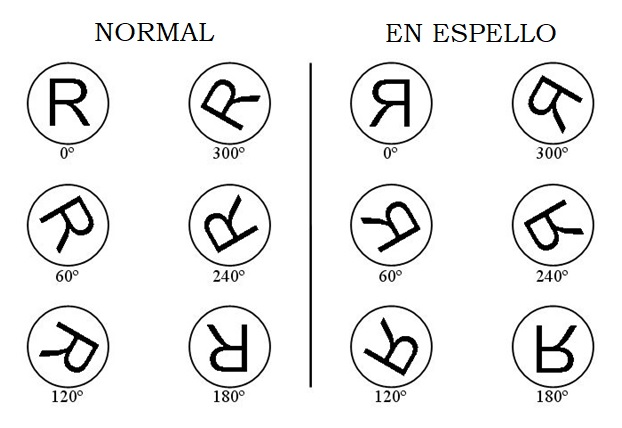
\includegraphics[width=0.5\linewidth]{memoria5_1}}
	\subfigure[Condicións experimentais]{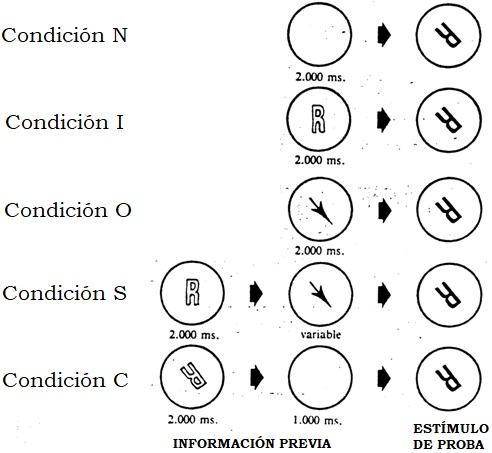
\includegraphics[width=0.45\linewidth]{memoria5_2}}
\end{figure}

Este paradigma plantea unha serie de cuestións: 
\begin{itemize}
	\item[•] Por que non existe unha relación lineal entre o ángulo de orientación e o TR?
	\begin{itemize}
		\item[] A ausencia de linealidade parece relacionarse coa familiaridade da orientación dos 
		estímulos. Cando só se desvían un pouco da orientación normal resultan máis familiares, e a 
		velocidade de rotación é maior que en orientacións máis alonxadas da normal.
	\end{itemize}
	\item[•] A rotación en imaxes só ocorre nun espazo bidimensional ou hai rotacións en 
	profundidade?
	\begin{itemize}
		\item[] Shepard e Metzler (1971) obtiveron evidencia experimental de se poden rotar imaxes 
		de obxectos tridimensionais.
	\end{itemize}
\end{itemize}

Pode concluirse desta investigación que as imaxes mentais de tipo visual parecen ocupar algunha forma de espazo mental, do mesmo xeito que os obxectos ocupan espazo físico no mundo real. As imaxes poden someterse a transformacións mentais, estruturais e funcionais análogas á rotación física dun obxecto real. 

\subsubsection{Desprazamento mental}
Estas investigación traballan con outros fenómenos que amosan o carácter espazo-temporal das imaxes. Baséanse en que a exploración dunha imaxe mental se ve facilitada polo seu tamaño, e en que o tempo de desprazamento mental dunha parte da imaxe a outra depende da distancia entre elas. 

Kosslyn (1978) basea as súas investigacións na preservación de distancias nas imaxes mentais: se estas son analóxicas, manterán as distancias relativas entre os detalles do obxecto ou escea imaxinado, e en consecuencia o tempo empregado nos desprazamentos relacionarase coas distancias entre os puntos dun mapa aprendido previamente. 

Os suxeitos comezan estudando o mapa dunha isla imaxinaria, que contén sete localizacións diferentes. O mapa apréndese contrastando a imaxe mental coa figura real, ata conseguir xerar unha imaxe precisa. Por último, os suxeitos debuxan as sete localizacións e compárase o debuxo co mapa repetidas veces ata obter unha imaxe precisa.

Na segunda fase, o suxeito situarse mentalmente nun punto do mapa. Proporciónaselle unha palabra que se refire a un punto distinto do mapa ou que non ten que ver con el. No primeiro caso, o suxeito debe desprazarse mentalmente, o máis rápido posible, desde o punto no que está ata o que se lle indica, o logo pulsar un botón. No segundo caso debe pulsar un botón diferente.

Os resultados amosan que o tempo que dura o desprazamento mental mantén unha relación lineal coa distancia en centímetros entre os puntos. A correlación entre ambos parámetros é case perfecta (0,97). Estes datos suxiren que as imaxes mentais non son epifenómenos, senon entidades cuasi-pictóricas que preservan as distancias.

Pinker (1980) aporta evidencia de que as distancias se manteñen nun espazo mental tridimensional. Os suxeitos aprenden a elaborar unha imaxe mental nítida e precisa dunha caixa con varios xoguetes, suspendidos do teito a varias alturas e profundidades. Logo realizan ensaios nos que se mide o tempo de diversos desprazamentos entre pares de obxectos. De novo, o TR correlaciona coa distancia na terceira dimensión. 

Posteriormente xorden varias críticas en torno á validez interna destes estudos. En primeiro lugar, crese que as investigacións están suxeitas ás características da demanda: os suxeitos deducen o propósito da investigación e manipulan as súas respostas para adaptalas ós resultados procurados, ou ben saben, pola súa experiencia previa, que percorrer visualmente unha distancia maior leva máis tempo que recorrer unha curta, e acomodan as súas latencias de resposta a este coñecemento implícito.

Por outra banda, as imaxes son permeables á información semántica, isto é, os fenómenos poden verse modulados polo coñecemento proposicional ou conceptual dos suxeitos.

\subsubsection{Inspección de imaxes}
Ademais de preservar as distancias relativas, o carácter análogo espacial das imaxes mentais tamén lles permite reflexar e modificar o tamaño dos obxectos, achegándoos ou afastándoos. Como consecuencia disto, é máis difícil detectar un detalle visual nunha imaxe pequena que nunha grande, igual que ocorre na percepción de obxectos reais. 

Para estudar este fenómeno, Kosslyn (1975, 1976) realiza experimentos nos que fai variar o tamaño dunha imaxe mental dos seus suxeitos para medir o tempo que tardan en detectar un detalle nela. En cada ensaio, os suxeitos reciben o nome de dous animais (o primeiro deles sempre é unha mosca ou un elefante) dos que deben xerar, a partir de instrucións, unha imaxe mental de ambos xuntos proxectados nunha parede blanca. Logo infórmaselles dunha propiedade relativa ó animal crítico, que deben visualizar o máis rapidamente posible para poder apretar un interruptor. 

Os resultados amosan un maior número de erros e latencia de resposta no contexto do elefante que no da mosca. Isto indica que o contexto determina o tamaño subxectivo do animal crítico, o que corrobora a hipótese de que as imaxes mentais preservan analoxicamente o tamaño dos obxectos.

\subsection{Mapas cognitivos}
\subsubsection{Aproximación de laboratorio \textit{versus} aproximación ecolóxica}
Fronte á investigación baseada en tarefas artificiais de laboratorio, os estudos de coñecemento ambiental analizan a información que temos as persoas sobre o noso entorno físico. Neste contexto, as imaxes mentais estudanse desde unha perspectiva ecolóxica, tratando de describir os mapas cognitivos que elaboramos acerca do noso entorno para orientarnos nel e ser quen de describilo. 

O termo <<mapas cognitivos>> procede de Tolman, pero será Lynch quen renovará a investigación con eles. Comeza entrevistando a algúns habitantes de varias cidades americanas, pedíndolles que debuxen mapas esquemáticos destas. Desta información extrae varios tipos de elementos que configuran a imaxe cognitiva da cidade:
\begin{itemize}
	\item \underline{Hitos}: Lugares con gran saliencia visual que adoitan tomarse como puntos de 
	referencia (catedral, prazas, fontes, etc.).
	\item \underline{Traxectos}: Liñas de tránsito que unen puntos de referencia e teñen especial 
	preponderancia para o cidadán (algunhas rúas).
	\item \underline{Distritos ou barrios}: Áreas da cidade que son cognitivamente homoxéneas (zona 
	vella, zona nova, campus sur, campus norte...).
	\item \underline{Nodos}: Puntos de importancia estratéxica na cidade, onde adoitan confluir os 
	traxectos (rotondas, esquinas, etc.).
	\item \underline{Bordos}: Límites aparentes de distritos ou zonas (ríos, murallas...).
\end{itemize}

\subsubsection{O concepto de mapa cognitivo}
\begin{itemize}
	\item \textbf{Metáfora do mapa:} Non debe interpretarse literalmente. O mapa cartográfico non é 
	unha copia literal da xeografía, senon un modelo axustado. Reflexa só algúns parámetros da 
	realidade, xera distorsións nas pautas espaciais e só adquire sentido pleno e funcionalidade 
	cando quen o le é quen de interpretalo correctamente. Implica unha dualidade estrutura-proceso, 
	sendo a primeira variable física, e a segunda, esencialmente cognitiva. Polo tanto, a do mapa 
	cartográfico non é a metáfora máis esclarecedora para explicar o noso coñecemento ambiental.
	\item \textbf{Mapa cognitivo como proceso:} O mapa cognitivo non é unha estrutura acabada e 
	estática, senon un proceso construtivo de razoamento espacial que permite resolver multitude de 
	problemas de localización, orientación, comprensión e desprazamento. É flexible e dinámico, e 
	ten un carácter multimodal, en tanto que o seu compoñente imaxinativo está modulado por 
	información conceptual e proposicional.
\end{itemize}

\subsubsection{Investigacións empíricas}
\begin{itemize}
	\item \underline{Dificultades metodolóxicas}: O mapa cognitivo é unha representación interna, 
	polo que é difícil exteriorizalo. O procedemento máis sinxelo e natural para facelo é 
	entrevistar ós suxeitos ou pedirlles que realicen mapas esquemáticos, que ofrecen información 
	moi rica sobre a imaxe mental dos individuos sobre o seu entorno pero presentan algúns 
	inconvintes. Dependen en gran medida da destreza no debuxo dos suxeitos e non teñen por que 
	reflexar a súa representación cognitiva: o mapa é un modelo feito segundo certas convencións 
	culturais que se reflexan na súa comprensión e execución, pero algúns individuos non os coñecen 
	e desenvólvense perfectamente no seu entorno.
	\item \underline{Estimación de distancias}: 
	\begin{itemize}
		\item \textbf{Evans e Pezdek (1980):} Os suxeitos deben estimar a que par de lugares 
		corresponde unha maior distancia. O TR garda unha relación lineal co grao de disparidade 
		entre as distancias comparadas, isto é, a resposta é máis rápida canto máis diferentes son 
		as distancias. Isto indica que os mapas cognitivos preservan as distancias métricas ó modo 
		característico das imaxes mentais (aínda que, en realidade, só se reteñen en formato 
		analóxico as relacións espaciais máis estratexicas; o contrario implicaría unha sobrecarga 
		para o noso sistema cognitivo, polo que o resto de xuizos baséanse en procesos de inferencia 
		e razoamento).
		\item \textbf{Byrne (1979):} Os suxeitos estiman as distancias entre puntos dunha cidade, e 
		obtense que as rutas do centro se estiman máis longas do que son (cousa que non sucede coa 
		periferia) e que xulgan máis longas as rutas con curvas que con rectas. Os resultados 
		reflexan un sesgo na estimación de distancias: cantos máis puntos hai nunha ruta, máis longa 
		se estima.  
		\item \textbf{Sadalla (1980):} Prodúcense asimetrías que amosan que a estimación da 
		distancia de ida dun punto a outro (A-B) non sempre coincide coa de volta (B-A), o que se 
		debe á preponderancia relativa dos lugares: o coñecemento espacial organízase en torno ós 
		lugares máis prototípicos, que sirven de referencia e cuxas relacións espaciais se almacean, 
		e os demais lugares interfiren na relación con estes. Este sistema maximiza a economía 
		cognitiva ó evitar sobrecargar a memoria cunha complexa representación de tódalas relacións 
		espaciais. 
	\end{itemize} 
	\item \underline{Estimación de orientación}: 
	\begin{itemize}
		\item \textbf{Wilton (1979):} Os xuizos sobre a posición relativa de pares de lugares son 
		máis rápidos cando estas pertencen a países ou rexións diferentes. O coñecemento xeográfico 
		parece organizarse xerarquicamente. 
		\item \textbf{Stevens e Coupe (1978):} Prodúcense distorsións nos xuizos espaciais cando 
		existe unha incongruencia entre a posición relativa de dúas cidades e a situación das súas 
		unidades xeográficas supraordinadas. 
		\item \textbf{Lynch (1960):} O coñecemento prototípico dos lugares afecta á nosa imaxe do 
		medio, de forma que os esquemas xerais distorsionan as imaxes particulares. 
		\item \textbf{Tversky (1981):} Na codificación e recordo de relacións espaciais xeográficas 
		empréganse dous heurísticos:
		\begin{itemize}
			\item \underline{Heurístico de aliñamento}: Relaciónase co agrupamento perceptivo. Da 
			lugar a que as unidades xeográficas tendan a situarse en liña, aínda que a súa posición 
			correcta sexa máis irregular.
			\item \underline{Heurístico de rotación}: Relaciónase co importante papel dos eixos 
			cartesianos na nosa percepción. A experiencia perceptiva organízase en torno á vertical, 
			definida pola gravedade, e á horizontal, definida polo horizonte. 
		\end{itemize}
	\end{itemize}
\end{itemize}

\subsubsection{Conclusións}
Destacamos certas propiedades que emerxen dos estudos actuais sobre o mapa cognitivo:
\begin{itemize}
	\item \textbf{O mapa cognitivo como representación multimodal:} Algunhas relacións espaciais 
	represéntanse de forma imaxinativa, e a información espacial organízase categorialmente e está 
	modulada por esquemas cognitivos. 
	\item \textbf{O sistema euclidiano non é un bo modelo dos mapas cognitivos:} O mapa cognitivo 
	non é unha estrutura ríxida de relacións espaciais. Nel, as distancias e orientacións fluctúan 
	considerablemente en función de parámetros contextuais e semánticos.
	\item \textbf{O mapa cognitivo inclúe procesos de razoamento espacial:} Ademais dun sistema de 
	coñecementos conceptuais e representacións analóxicas, o mapa é un sistema de resolución de 
	problemas, un conxunto de regras que permiten facer inferencias.
	\item \textbf{O mapa cognitivo axústase a un principio de economía:} As representacións 
	espaciais do mapa son livianas e imprecisas para evitar unha sobrecarga de memoria. Con todo, o 
	sistema cognitivo compensa estas imprecisións cunha maior cantidade de procesamento.
	\item \textbf{O mapa cognitivo satisfai demandas adaptativas:} O mapa cognitivo presenta 
	múltiples ``imperfeccións'' e sesgos. Pero posúe un gran valor adaptativo se temos en conta a 
	enorme eficiencia da nosa conduta espacial. Isto suxire que os procesos cognitivos subxacentes ó 
	mapa son suficientemente ``precisos'' e ``correctos''.
\end{itemize}

\end{document} %Non pode haber nada escrito despois desta instrución.
